\Section{Deep Learning, Normalizing Flows and Invertible Neural Networks}
\label{sec:deeplearning}

Deep Learning is a subdomain within Machine Learning focussing on the construction and training of deep neural networks. Such networks have been proven to be extremely successful in different, analytically unsolvable problems such as (but not restricted to) image classification tasks, regression tasks, image generation tasks, language translation and reinforcement learning.

In this chapter, a brief introduction to these networks and their properties with a focus on so-called normalizing flows and invertible neural networks is given.

\Subsection{Foundations of Deep Learning and Neural Networks}
\Subsubsection{The Universal Approximation Theorem}

The success of Neural Networks (NNs) lies in their potential of learning (almost) arbitrary models. This property of NNs can be expressed mathematically through the Universal Approximation Theorem which in words states \cite{DLiPR}:

\begin{quote}
	\centering
	A feed-forward network with linear output and at least one hidden layer with a finite number of nodes can approximate any real continuous function on a given closed and bounded subset to arbitrary precision.
\end{quote}

However, the Universal Approximation Theorem does not state how the network should be constructed to achieve the desired precision. For this reason, the theorem has been proven for several network architectures; in case of ReLU-activated feed-forward networks the theorem can be written as the following \cite{UAC}:
\newtheorem{theorem}{Theorem}
\begin{theorem}
	For any real and continuous function $f : [0, 1]^{d_{in}} \rightarrow \mathbb{R}^{d_{out}}$ and every $\epsilon>0$ there is a ReLU-network $\mathcal{N}$ with the same input and output dimension $d_{in}$ and $d_{out}$ and hidden layer width at most $w$ for which
	\begin{equation*}
		\sup_{x\in[0, 1]^{d_{in}}}\Vert f(x)-f_\mathcal{N}(x)\Vert \leq \epsilon
	\end{equation*}
	and
	\begin{equation*}
		d_{in} + 1 \leq w_{min}(d_{in}, d_{out}) \leq d_{in} + d_{out}
	\end{equation*}
\end{theorem}
This theorem does not state anything about the exact depth (number of layers) the network needs to have, its speed of convergence and the optimization process it needs to undergo to achieve this arbitrary approximation. On the other hand, it is reassuring to have a mathematical guarantee for convergence for a given feed-forward network structure. For this reason, empiric studies are usually performed to look for a locally optimal solution for a given task.

In the following, a brief overview of the most common NN components is going to be given with special focus on the ones used for the construction of the cINN.

\Subsubsection{Fully-Connected Neural Networks}
The most elementary NNs perform affine transformations (consisting of a linear transformation represented by a matrix $W$ and a shift $b$) on a given input $x$ followed by the application of a non-linear function (called activation) $g$:

\begin{equation*}
	y = g(Wx+b)
\end{equation*}

Graphically, one such transformation is represented as a layer. For a fully-connected neural network, these transformations are called in succession, resulting in stacked layers of $n$ nonlinearities as shown in fig. \ref{fig:nn}. The resulting mapping

\begin{equation*}
	f(x, \theta) = g^n\left\{W^{n-1}g^{n-1}\left[ ... \left(W^2g^1(W^1x+b^1)+b^2\right)...\right]+b^{n-1}\right\}
\end{equation*}

is a universal approximator with the free parameters $\theta$ (containing all the matrices $W^i$ and the biases $b^i$) for the target output for $y$. Finding the optimal parameters $\theta$ is called training and the $\theta$ will be referred to as trainable parameters.

\tikzset{%
	every neuron/.style={
		circle,
		draw,
		minimum size=1cm
	},
	neuron missing/.style={
		draw=none, 
		scale=2.5,
		text height=0.333cm,
		execute at begin node=\color{black}$\vdots$
	},
}
\begin{figure}[h!]
	\centering
	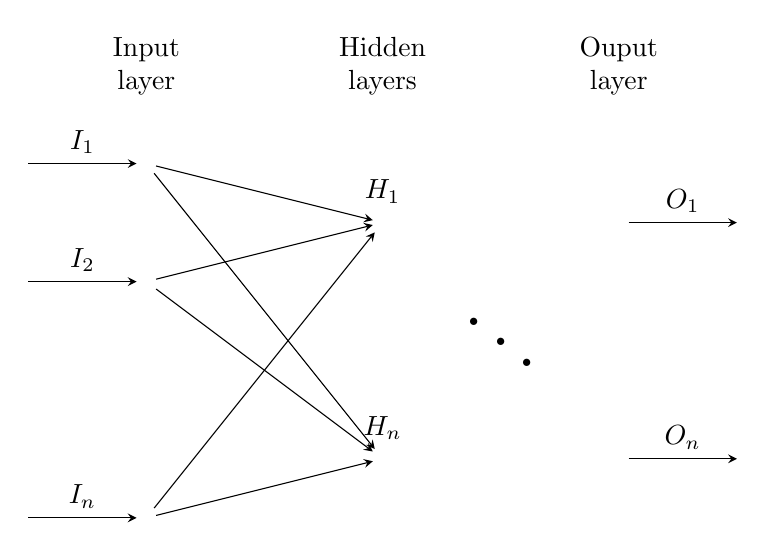
\begin{tikzpicture}[x=1.5cm, y=1.5cm, >=stealth]
		
		\foreach \m/\l [count=\y] in {1,2,missing,3}
		\node [every neuron/.try, neuron \m/.try] (input-\m) at (0,2.5-\y) {};
		
		\foreach \m [count=\y] in {1,missing,2}
		\node [every neuron/.try, neuron \m/.try ] (hidden-\m) at (2,2-\y) {};
		
		\foreach \m [count=\y] in {1,missing,2}
		\node [every neuron/.try, neuron \m/.try ] (output-\m) at (4,2-\y) {};
		
		\foreach \l [count=\i] in {1,2,n}
		\draw [<-] (input-\i) -- ++(-1,0)
		node [above, midway] {$I_\l$};
		
		\foreach \l [count=\i] in {1,n}
		\node [above] at (hidden-\i.north) {$H_\l$};
		
		\foreach \l [count=\i] in {1,n}
		\draw [->] (output-\i) -- ++(1,0)
		node [above, midway] {$O_\l$};
		
		\foreach \i in {1,...,3}
		\foreach \j in {1,...,2}
		\draw [->] (input-\i) -- (hidden-\j);
		
%		\foreach \i in {1,...,2}
%		\foreach \j in {1,...,2}
%		\draw [->] (hidden-\i) -- (output-\j);
%		\draw [->] (hidden-1) -- (output-1);
%		\draw [->] (hidden-2) -- (output-2);
		
		\foreach \l [count=\x from 0] in {Input\\ layer, Hidden\\ layers, Ouput\\ layer}
		\node [align=center, above] at (\x*2,2) {\l};
		
		\node [draw=none, scale=2.5, text height=0.333cm] at (3, 0) {$\ddots$};
		\node [draw=none, scale=2.5, text height=0.333cm] at (3, 1.25) {$\hdots$};
		\node [draw=none, scale=2.5, text height=0.333cm] at (3, -0.75) {$\hdots$};
		
	\end{tikzpicture}
	\caption{Schematical structure of a feed-forward NN. The nodes represent the variables for the hidden and output layers or the biases applied to the intermediate outputs for the hidden layers. Arrows represent the matrix $W$ and the activations $g$.}
	\label{fig:nn}
\end{figure}

Note that for the approximation to work arbitrary well, the structure of the network and training have to be correctly adjusted to the task to be solved.

\Subsubsection{Activation Functions}
It is essential for convergence to select the right activation function $g$. Historically, several candidate activation functions such as sigmoid, tanh, the rectified linear unit (ReLU) and its variants such as SeLU and leaky-ReLU have emerged. In this work ReLU will be used exclusively. One great advantage of ReLU is the lack of saturation range compared to the sigmoid or tanh activation functions, where gradients above or below a given value of $x$ become negligible, "paralysing" the training. Apart from that, ReLU has tractable derivatives and has proven to be an efficient activator empirically. It is defined as

\begin{equation*}
	\text{ReLU}(x) = \max \{0, x\}
\end{equation*}

where the maximum is taken element-wise over the vector components of $x$. Note that its derivative is not continuous and makes a jump at the origin from 0 to 1, which unnecessarily renders parameters 0 during training. On the other hand, this activation function has no scale, making it an excellent candidate for general approximation tasks. A graph of the most commonly used activation functions is shown in fig. \ref{fig:activations}.

\begin{figure}
	\centering
	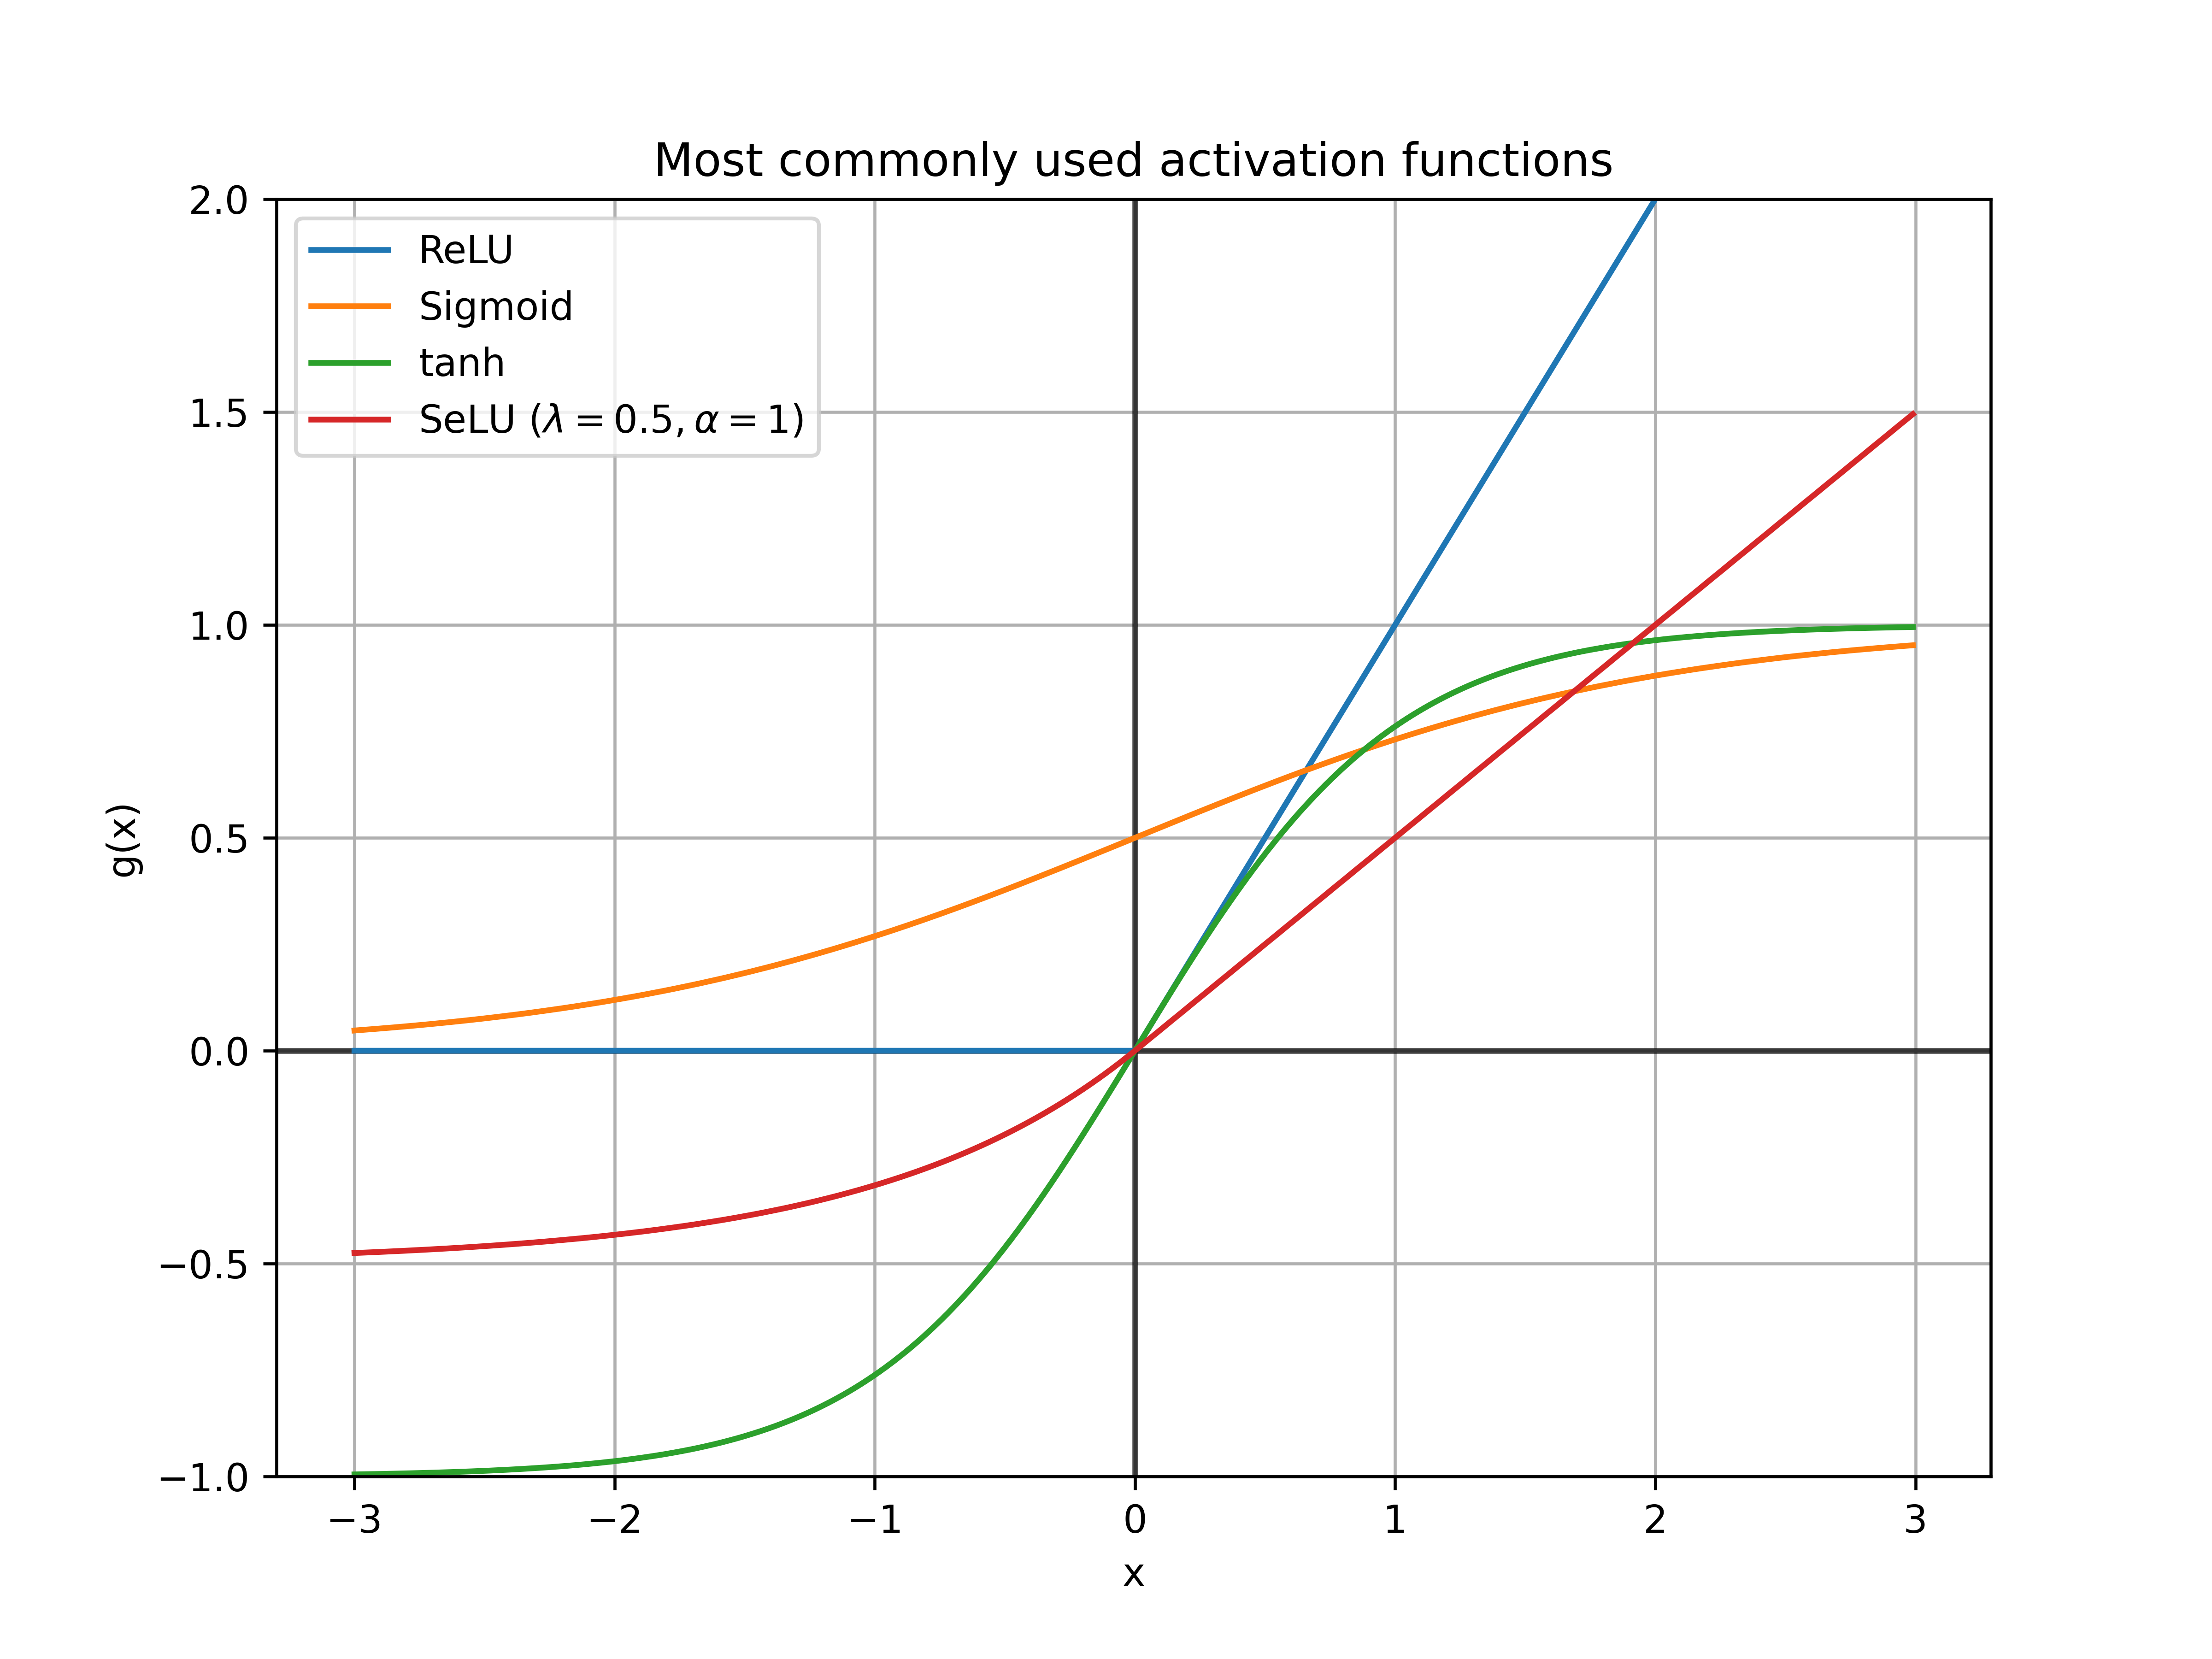
\includegraphics[width=0.7\linewidth]{figures/neural_networks/activations}
	\caption{Most commonly used activation functions. Note the plateaus of the sigmoid and tanh functions and for all $x<0$ for ReLU. Setting the gradient zero for x<0 renders several parameters inactive during training; on the other hand, large positive parameters have do not get stuck due to vanishing gradients and the function is scaleless}
	\label{fig:activations}
\end{figure}



